\subsection{Instrumentation Amplifier:}

For the circuit in Figure 3.2.0 we simulate it and captured in Figures 4.2.0 and 4.2.1, the results of the measures where registered in Table 4:

\begin{figure}[H]
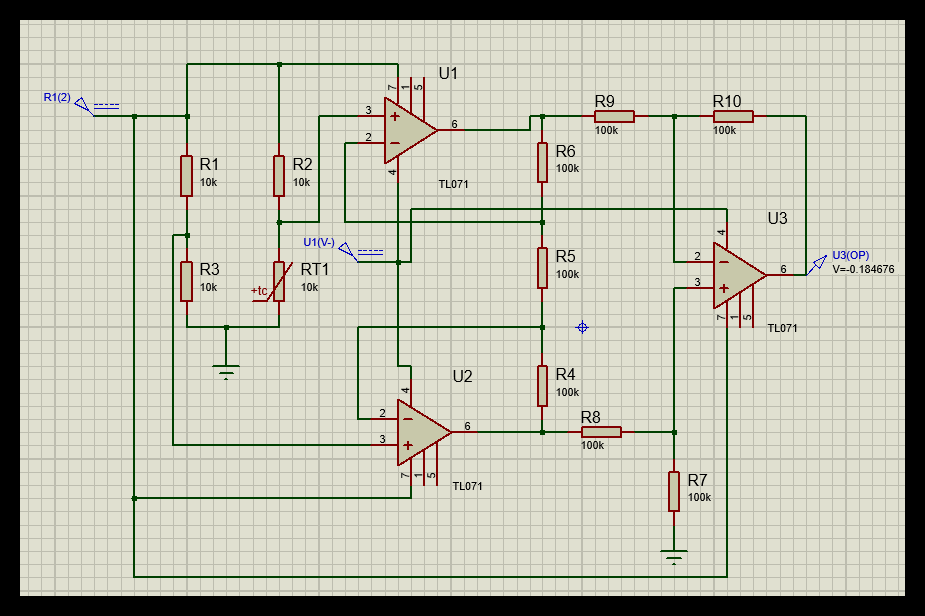
\includegraphics[width = 16.5cm, height = 8cm]{ia.png}
\centering \linebreak \linebreak Figure 4.2.0: Instrumentation amplifier with thermistor in ambient temperature.
\end{figure} \hfill

\begin{figure}[H]
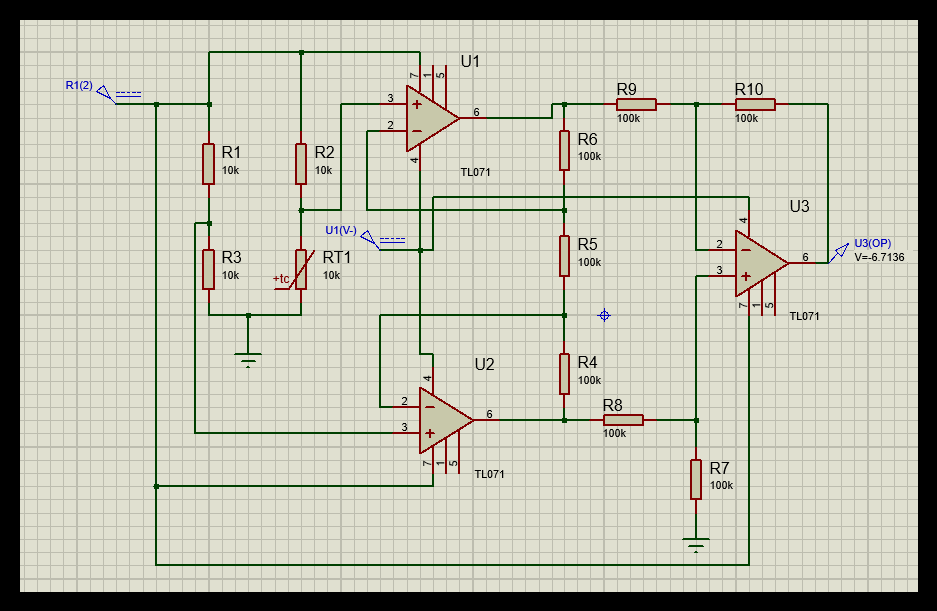
\includegraphics[width = 16.5cm, height = 8cm]{ie.png}
\centering \linebreak \linebreak Figure 4.2.1: Instrumentation amplifier with thermistor in high temperature.
\end{figure} \hfill

\begin{center}
\begin{tabular}{c c}
\toprule \toprule
\hspace{80px} Temperature \hspace{80px} & \hspace{80px} Output Voltage \hspace{80px} \\
\midrule \midrule
Ambient & 0.18 V \\
\cmidrule{1-2}
Putting a lighter close & 6.71 V \\
\bottomrule
\end{tabular}
\linebreak \linebreak Table 4: Figures 4.2.0 and 4.2.1 measured values.
\end{center}

\pagebreak